\chapter{History}\label{ch:history}

\begin{wrapfigure}{R}{0.3\textwidth}
\centering
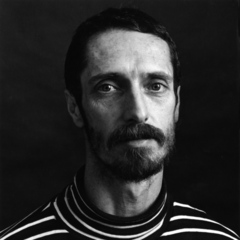
\includegraphics[width=0.25\textwidth]{images/history}
\end{wrapfigure}

``\textit{To know who you are today, I need to know your past, and maybe even can predict something about your future.}''
This applies not only to individuals, but as well to humanity as a whole and localized phenomena like the art of CI itself.
By knowing its origins, we can prevent from diverting too far from it, and reach a more profound understanding of why things are the way they are.
And also, of course, to bring in some kind of attitude of honor, paying our respect to the founding fathers -- and mothers.
To bring in some tradition; something our society these days so much lacks and yet is so much in need of -- even though it might not be aware of it.

\section{Founding Parents}\label{sec:founding-parents}

CI was developed in June \textbf{1972} in the US by mainly a man called \textbf{Steve Paxton}, ``the father of CI'' -- see his picture on the right --, who was an American dancer, gymnastics and choreographer and former Aikidoka (someone who practices the Japanese martial art Aikido) who lived in New York City (by that time mainly performing in the Judson Dance Theater).
He was keen to explore and push the boundaries to develop this new practice, some sort of ``art-sport''.

Next to him, it is worth mentioning \textbf{Nancy Stark Smith} -- ``the mother of CI'' --, who is the one still holding CI, as Steve stopped doing CI about 7 years after its invention, intenting to give it to the people.
She continued with another partner and started the Contact Quarterly magazine, a vehicle to share ideas, to hold the theme and practice of CI\@.

\section{Creation}\label{sec:creation}

In spring 1972, Steve Paxton invited a group of 17 students and colleagues, dancers, martial artists, acrobats, gymnasts and athletes, to explore and research the \textbf{extremes of movement and disorientation} -- from standing still to falling, rolling, colliding and jumping in the air -- in a two-week workshop.
While moving with high velocity, running into each other, bumping, trying to survive, and see what the result will be.\footnote{A little bit like what they do at the Large Hadron Collider at CERN: Smashing some particles at each other and be excited about what would happen.}

He wanted the dancers to work with him on the form he was evolving, and at the end of this week of residency, the group presented a performance named ``Contact Improvisation''.
To see for yourself how those first steps looked like, watch this old black-white recording from 1972: \url{https://www.youtube.com/watch?v=9FeSDsmIeHA}

Out of that exploration, a 20-minutes performance piece called ``\textit{Magnesium}'' arose, whereas the first quarter-hour was about jumping and bumping, manipulation and clinging.
Only the last 5 minutes, the so-called ``\gls{smalldance}'' was performed: A form of meditation that is practiced standing, where attention is paid to postural adjustments and micro-weight transfers.
Videos narrated by Steve about that are available, which are very much encouraged to watch, to also see the progression from those impactful years of '72, '75 and '87.

\section{Institutionalization}\label{sec:institutionalization}

At first, around 1975, it was considered to \textbf{trademark} the term Contact Improvisation, but this idea was rejected in favor of establishing a forum for communication, which nowadays is the website of \href{https://contactquarterly.com}{Contact Quarterly} and is still co-edited by Nancy Stark Smith herself.
So it was never \textbf{institutionalized}, nor was the name \textbf{copyright} protected.
Together with \href{http://www.ecite.org}{ECITE} (the European Contact Improvisation Teachers Exchange), those two can be considered the main international forums ensuring the quality and continuation of CI\@.

The decision was very deliberate to not have any form of legal institute or \textbf{certifications}, free of any hierarchy.
Remember that a certificate usually doesn't mean that that person is good, but just that the certification was passed.

The downside of not having an authority verifying the competence of the teachers is, of course, that when the word was spreading, more and more \textbf{injuries} started to happen; that's why: ``\textit{One should never teach what one doesn't know properly}''.

\section{Further Spreading}\label{sec:further-spreading}

A few years after the founding event, the very first ``Country Jam'' was organized in 1979, where about 50 people came together to freely exchange and dance, without any structure.
Neither a workshop, conference nor a seminar.
Just co-created being, dancing and living in flux.
Later on, it was introduced in new avant-garde (experimental artists) dance schools in the US\@.

The members of the founding group scattered across the US and started to teach the practice.
It became smoother, continuous and \textbf{controlled}, yet still avoiding eye and direct hand contact.
Much emphasize was put on the experience of flow, which is more of an aesthetic choice (Nancy Stark Smith), yet the central characteristics preserved.

\textbf{Europe} was presented with CI first 1873 in Italy, and later Steve Paxton and Lisa Nelson regularly went to the UK and Amsterdam (School for New Dance Development) as the transmission belts for CI in the whole of Europe.
Belgium was visited by Paxton since the 1980s, but apart to certain outbreaks of fever in successful jams, it didn't leave any lasting traces among dancers.

As founding people could be considered (next to Steve Paxton): Nancy Stark Smith, Danny Lepkoff, Lisa Nelson, Karen Nelson, Nita Little, Andrew Harwood, and Ray Chung.

For more detailed information, read books like \textit{Sharing the Dance} and others which you can find in the~\nameref{ch:resources} section.

\section{Then and Now}\label{sec:then-and-now}

It was, for sure, very different back then, and that's why sometimes people would also refer to it as ``\textit{Old School Contact}''.
There was a \textbf{high risk} with very high velocity, and it, for sure, looked very amazing -and very scary too.
Good to know, though is, that they trained on \textbf{mats}, especially at the very beginning (see the videos), which would make the impact of falling much less.
After they started to do the same without mats, though, they got -- quite a lot of -- injuries.

In the last few decades, much more emphasis was put on \textbf{flow}, instead on ``explosion'', and also on figuring out the \textbf{least resistant} pathway.
Some people claim that CI lost quite a lot of its characteristics along the way, yet it could be said that it's nice to have both, to be able to choose what you want.
Being able to survive the explosion, and play comfortably in the flow.

Today there are many different \textbf{styles}: more flow, more impactful, acrobatics, dance, acting, \ldots
The differences are mostly based on the uniqueness of the teachers, along with their lineages; but also due to culturally specifics.
Some countries may have simply other ``body orientations'', resulting in a different CI style.

\section{Future}\label{sec:future}

Hopefully, it will keep a \textbf{strong trunk}, meaning: People keep on researching the practice, while still knowing where it comes from, knowing its roots.
We are all welcoming the \textbf{branches}, e.g.\ CI combined with other practices like ``Contact Tango'', ``Contact Beyond Contact'', and so forth, or CI with using substances for \textit{other states of awareness}.
Hoping for -- as the tree is branching -- that the main trunk will stay the main trunk so that there is no need for the distinction between ``I am a CI \textit{purist}'' but that it's possible to simply say: ``I'm doing CI''.
The trunk has been \textbf{stable} for the last 50 years, yet plenty of new branches appeared in the last 20 years; branches which merge different forms together.
It is important that people be aware that those branches and merges are not CI the way it is actually practiced.
And lastly, what's needed are good teachers, jams, and spaces where the ideas and principles are held from CI: Knowing the physical aspect but also keeping the history.
